\documentclass[10pt,a4paper]{article}
\usepackage{graphicx}
\usepackage[a4paper, total={6in, 9in}]{geometry}
\graphicspath{ {/} }
\usepackage{amsmath}
\usepackage{algorithm}
\usepackage[noend]{algpseudocode}
\usepackage{enumerate}

\makeatletter
\def\BState{\State\hskip-\ALG@thistlm}
\makeatother

\begin{document}
	
	\section*{Problem 1}
	
	
	
	\section*{Problem 2}
	
	\begin{itemize}
		\item
		A. 
		\begin{center}
			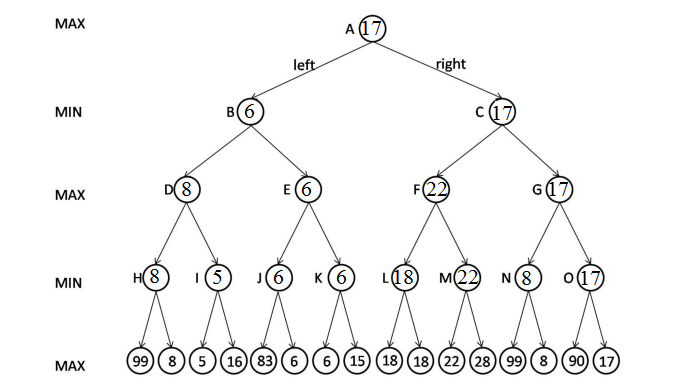
\includegraphics[scale=0.5]{Minimax}
		\end{center}
		\item
		B. 
		\begin{center}
			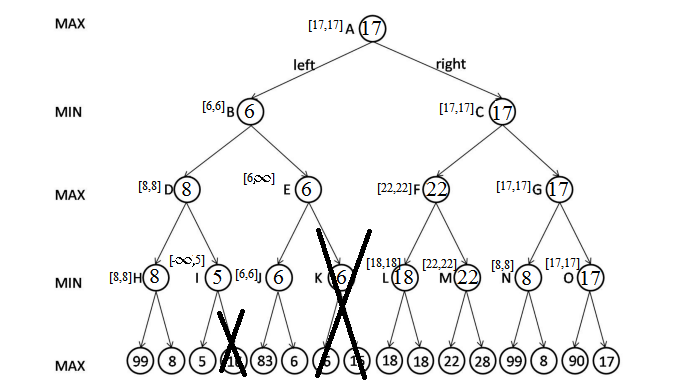
\includegraphics[scale=0.5]{Pruning}
		\end{center}
		
		We cut off the subtree at node K since node B is a MIN and will only accept a value less than 8 we know that we wont get a value greater than 6 down said subtree. The same also occurs below node I. The terminal node 15 is pruned because node D will accept any number greater than 8 however, node I is a MIN and the left terminal node being 5 allows us to denote that the right terminal node cannot be less than 5.
		
		\item 
		C. The max player will choose 17 at the root state by using the exhaustive Minimax Algorithm. The same result will occur when using alpha-beta pruning
		and the max player will again choose 17. The most optimal move is guaranteed using either the exhaustive Minimax algorithm or the alpha-beta pruning algorithm. This is accomplished by alpha-beta pruning ignoring subtrees that are irrelevant while exhaustive Minimax algorithm checks every node regardless of relevance. The outcome is the same however, since alpha-beta pruning ignores irrelevant subtrees it is more efficient.
		
		\item
		D. 
		
		\item
		E. 
	\end{itemize}
	\clearpage
	\section*{Problem 3}

	
	\begin{enumerate}[A.]

		\item
		
		\textbf{Variables:} Defined as $n_{i,j}$ where $i \in \text{\{set of all row numbers\}}$ and $j \in \text{\{set of all column numbers\}}$ for each cell $n$ on the board. Essentially, each square on the sudoku board will be a variable, for a total of 81 variables.
		
		\textbf{Domain:} Defined as the set of possible values in sudoku. Here, this set is defined as $\{ 1, 2, ..., 9 \}$
		
		\textbf{Constraints:}
		
		\begin{enumerate}[1.]
			\item All variables in any row must be assigned distinct values.
			\item All variables in any column must be assigned distinct values.
			\item All variables in any 3x3 region must be assigned distinct values.
			\item The assignments given to variables in the start state cannot be changed.
		\end{enumerate}
		
		\item
		
		\textbf{Start State:} The start state is a given board that has variables assigned with certain values. These values are the basis for the constraints for the rest of the problem and may not be changed. Below is an example start state.
		
		\begin{center}
			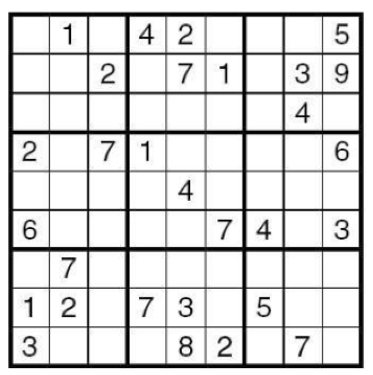
\includegraphics[scale=0.4]{sudoku_startstate}
		\end{center}
		
		\textbf{Successor Function:}  
		
		\begin{enumerate}[1.]
			\item Select a random unassigned variable 
			\item Assign a value to this variable that does not violate any constraints
			\item The resulting state is the successor
		\end{enumerate}
		
		\textbf{}
		
		\item 

		\item Pseudocode for Local Search

		\begin{algorithm}
			\caption{Sudoku Local Search Algorithm}\label{euclid}
			\begin{algorithmic}[1]
				\Procedure{SudokuSolver}{$\text{Board}$ $\textit{board}$}
				\State $\textit{board} \gets \text{randomizeCompleteState(\textit{board})}$
				\While {$\text{!completeAndSatisfied(\textit{board})}$}
				\State $\textit{nextBoard} \gets \text{updateState(\textit{board})}$
				\If {$\text{evaluateSatisifiability(\textit{nextBoard})} > \text{evaluateSatisifiability(\textit{board})}$}
				\State $\textit{board} \gets \textit{nextBoard}$
				\EndIf
				\EndWhile
				\State $\text{return }\textit{board}$
				\EndProcedure
			\end{algorithmic}
		\end{algorithm}
		
	\end{enumerate}
	
    
	\section*{Problem 4}
	For Superman to be defeated, it has to be that he is facing an opponent alone and his opponent is carrying Kryptonite. Acquiring Kryptonite, however, means that Batman has to coordinate with Lex Luthor and acquire it from him. If, however, Batman coordinates with Lex Luthor, this upsets Wonder Woman, who will intervene and fight on the side of Superman.
	\begin{itemize}
	\item
	A.
	
	Superman defeated = S
	
	Facing Opponent Alone = A
	
	Opponent carrying Kryptonite = K
	
	Batman coordinates with Lex Luther = B
	
	Wonder Woman Upset = W
	
	\item
	B. Superman being defeated implies that not only did his opponent have Kryptonite but that Superman was also fighting alone. This is equivalent to Superman not being defeated or his opponent has Kryponite and Superman is fighting alone. This all equates to: 
	\begin{center}
		$(\neg S \lor K) \land (\neg S \lor A)$
	\end{center}
	
	Superman fighting alone implies that Superman was defeated. 
	\begin{center}
		$(\neg K \lor B)$
	\end{center}
	Batman coordinating with Lex Luther implies that Wonder Woman will be upset and will team up with Superman. 
	\begin{center}
		$(\neg B \lor W)$
	\end{center}
	Wonder Woman being upset implies that she will team up with Superman and he will not be fighting alone.
	\begin{center}
		$(\neg W \lor \neg A)$
	\end{center}
	\item
	C. Based off the knowledge presented above we can prove that Batman cannot defeat Superman. 
	
	\begin{center}
		$(\neg S \lor K) \land (\neg S \lor A) \land (\neg K \lor B) \land (\neg B \lor W) \land (\neg W \lor \neg A)$
		
		$(\neg S \lor \neg S) \land (\neg A \lor A) \land (\neg K \lor K) \land (\neg B \lor B) \land (\neg W \lor W)$
		
		$\neg S$
	\end{center}

	
	
	\end{itemize}
	
	\section*{Problem 5}
	\begin{itemize}
		\item
		A.
	\end{itemize}
	
	\section*{Problem 6}
	\begin{itemize}
		\item
		A. Using the minimum value of $h_1(n)$ and $h_2(n)$ for each state:
		
		\begin{center}
			Given that $h_1(n) \leq h^*(n)$ is always true, 
			
			$Min(h_1(n),$ $\infty) \leq h^*(n)$
		
			Therefore $h_1(n) = minimum (h_1(n), h_2(n))$ is admissible. 
			
			consistent? 
		
		\end{center}
		
		\item
		B. Using the maximum value of $h_1(n)$ and $h_2(n)$ for each state:
		
		\begin{center}
			
			Given that $h_1(n) \leq h^*(n)$
			
			$h_2(n) \leq h^*(n)$
			
			$Max(h_1(n),$ $h_2(n)) \leq h^*(n)$
			
			Therefore $h_4(n) = maximum(h_1(n),$ $h_2(n))$ is admissible.
			
			consistent? 
			
		\end{center}
		
		
		\item
		C. The defined heuristic function 
		\begin{center}
			$h_3(n) = w \times h_1(n) + (1-w)h_2(n),$ where $0 \leq w \leq 1$
		\end{center}
		
		is admissible only when w is a value less than 0.5, any value larger than 0.5 will cause $h_1(n)$ to be multiplied by a value larger than $h_2(n)$.  Since the the bounds are from 0 to 1 the heuristic is NOT admissible. 
			
			
			consistent? 
			
		
		
		\item
		D. Considering the informed, best-first search algorithm with an object function of $f(n) = (2-w) \times g(n) + w \times h(n)$. It is guaranteed to work for $0 \leq w \leq 1$ since being multiplied by g(n) which is a constant implies no effect on which order chosen paths are arranged. However, if $w > 1$, then the goal state may have an overestimated distance which will make the heuristic not admissible and so not optimal.
		
		Given the information above we can assess the function for when the values of w are 0, 1, and 2.
		
		$w = 0$:
		
		When $w = 0$ it will make $f(n) = 2g(n)$ and causes the algorithm to perform like a Uniform Cost Search since there is no weight assigned it will find the most optimal path however, it will not be efficient.
		
		$w = 1$:

		When $w = 1$ it will make $f(n) = g(n) + h(n)$ which causes the algorithm to perform like $A^*$ and as with $w=0$ is guaranteed to find the optimal path however, is more efficient.
		
		$w = 2$: 
		
		When $w = 2$ it will make $f(n) = 2h(n)$ which causes the algorithm to perform like Greedy Best first search.
		
	\end{itemize}
		
\end{document}